\documentclass[12pt]{article}
\usepackage[utf8]{inputenc}
\usepackage[english]{babel}
\usepackage{amsmath}
\usepackage{amssymb}
\usepackage{enumerate}
\usepackage{amsthm}
\usepackage{graphicx}
\usepackage{epstopdf}
\usepackage{hyperref}
\usepackage{textcomp}
\usepackage{caption}
\usepackage{subcaption}
\usepackage{microtype}
\usepackage{parskip}
\usepackage{float}
\usepackage{url}

\DeclareMathOperator*{\argmax}{arg\,max}
\DeclareMathOperator*{\argmin}{arg\,min}

\title{Brownian Bridges Movement Model}
\author{Quim Llimona, Universitat Autònoma de Barcelona}
\date{}

\begin{document}
\maketitle

\tableofcontents
\clearpage

%%%%%%%%%%%%%%%%%%%%%%%%%%%%%%%
%%%%%%%%%%%%%%%%%%%%%%%%%%%%%%%
\section{Introduction to Brownian Bridges}
%%%%%%%%%%%%%%%%%%%%%%%%%%%%%%%
%%%%%%%%%%%%%%%%%%%%%%%%%%%%%%%

Brownian Bridges (BB) are stochastic processes that describe beliefs on the position of a particle over time. They can be defined using the following stochastic Cauchy problem:

\begin{align*}
    p_t(x,t) &= \Phi(x) \\        % recheck definition of brownian motion
    p(x,t_1) &= \delta_1(x) \\
    p(x,t_2) &= \delta_2(x)
\end{align*}

where:

\begin{itemize}
    \item $x$ is the position vector
    \item $p(x,t)$ is the probability of being at position $x$ at time $t$
    \item $\Phi(x)$ is the dispersion kernel, and describes the distribution of an advance over space in a differential of time; we will assume it does not depend on time
    \item $t_1$ is the begin time of the bridge (often assumed to be 0)
    \item $t_2$ is the end time of the bridge
    \item $\delta_1(x)$ is a given pdf and describes where the particle can be at $t_1$
    \item $\delta_2(x)$ describes, likewise, where the particle can be at $t_2$, and is in some formulations equal to $\delta_1$ (circular bridges)
\end{itemize}

As can be deduced from the equations, BB model the behaviour of a particle whose dispersion kernel is known, and from which we know the position (or the distribution of it) at two time instants. The model is very useful when making computations within this time window; outside it, it reduces to the dispersion kernel $\Phi(x)$ integrated from the initial position $\delta_1(x)$ (for $t < t_1$) or from the final position $\delta_2(x)$ (for $t > t_2$).

From the model, lots of useful computations can be made; integrating over time, we can know the expected portion of time the particle spent in each point, and by further integrating over space we can know the expected portion of time the particle spent in a given are in a given period of time.

It is very common to use a Gaussian dispersion kernel, in which case the particle moves in Brownian Motion (hence the name of the model: the particle moves from one point to another using this kind of motion). In that case, there is a parameter to the model: $\sigma_m^2$, associated to how quickly the particle moves over space. Intuitively, the higher $\sigma_m^2$ is, the less we will know about its position at an intermediate time instant.

Regular Brownian Motion has a well-known solution of a Gaussian distribution centered at the origin and with increasing variance over time. Intuitively, Brownian Bridges should also have a Gaussian solution, where the variance increases with the distance (in time) to start and end, and the mean moves from the begin point to the end point.

%% give the formula here

% \begin{verbatim}
%     - generic bridge: any phi, any starting pdf
%     - brownian bridge: guassian starting pdf, brownian motion with given sigma_m
%     - what can we get from it? occupation time, plain pdf, etc
%     - mu and sigma interpolation, based on brownian motion
% \end{verbatim}

%%%%%%%%%%%%%%%%%%%%%%%%%%%%%%%
\subsection{Brownian Bridge Movement Model}
%%%%%%%%%%%%%%%%%%%%%%%%%%%%%%%

A very useful application of Brownian Bridges it the Brownian Bridge Movement Model (BBMM), which models where an animal can be in continuous time given a discrete set of observations in $(x,t)$ pairs. It constructs a Brownian Bridge between all pairs of consecutive observations, all with the same $\sigma_m^2$; when asked about a particular time instant $t$, the model picks the bridge corresponding to the two obervations $t$ lies in between and continues normally:

\[ p^*(x,t) = p_j(x,t), \quad t_j^1 < t \leq t_j^2 \]

where $p^*(x,y)$ is the BBMM output, $p_j(x,t)$ correspond to bridge built starting at observation with index $j$, $t_j^1$ is the begin time of bridge $j$, and $t_j^2$ is the end time of bridge $j$.

While in traditional Brownian Bridges $\sigma_m^2$ was a fixed parameter that had to be determined externally, in BBMM it is possible -- provided there is enough data -- to find that value as an optimization formulation within the model itself. For that, the only points with an odd index are used to building the bridges, and points with an even index are used for fitting $\sigma_m^2$. Given a BBMM and a set of fitting observations $(x_i,t_i)$, with $x_i$ a multi-dimensional position vector, the expected position of observation $i$ (that is, the probability that the particle is at position $x_i$ at time $t_i$) is equal to $p(x_i,t_i)$, for the bridge $t_i$ lies on. Therefore, the likelihood of our model given the fitting data is the joint probability of all observations given the parameter $\sigma_m^2$:

\[ L(\sigma_m^2 | (x,t)) = \prod_i p^*(x_i,t_i|\sigma_m^2) \]

Finding the optimal parameter $\hat{\sigma}_m^2$ reduces to:

\[ \hat{\sigma}_m^2 = \argmax_{\sigma_m^2} L(\sigma_m^2) \]

As we will show later, this can be computed through gradient descent-based minimization of the negative log-likelihood of the model ($-\log L$).

% \begin{verbatim}
%     - extension to N known, time-stamped points
%     - based on selecting the active BB as closest in time
% \end{verbatim}

%%%%%%%%%%%%%%%%%%%%%%%%%%%%%%%
\subsection{Other applications of Brownian Bridges}
%%%%%%%%%%%%%%%%%%%%%%%%%%%%%%%

Apart from Movement Ecology (BBMM), Brownian Bridges are best known for their application in Computational Finance. Instead of computing pdf's, as we have done here, they are used for generating simulated, realistic paths between two points efficiently. This allows methods similar to Monte Carlo simulation.

% \begin{verbatim}
%     - finance
% \end{verbatim}

\clearpage
%%%%%%%%%%%%%%%%%%%%%%%%%%%%%%%
%%%%%%%%%%%%%%%%%%%%%%%%%%%%%%%
\section{Implementation of a BBMM}
%%%%%%%%%%%%%%%%%%%%%%%%%%%%%%%
%%%%%%%%%%%%%%%%%%%%%%%%%%%%%%%

In this section we provide details for an efficient implementation of a Brownian Bridge Movement Model in the MATLAB language, suitable for simulations with real-world data.

%%%%%%%%%%%%%%%%%%%%%%%%%%%%%%%
\subsection{Estimation of $\sigma_m^2$}
%%%%%%%%%%%%%%%%%%%%%%%%%%%%%%%

As mentioned before, the optimal value of $\sigma_m^2$ can be computed through the minimization of the negative log-likelihood of the model. Let's formulate it first adding the normal distribution kernel (previously $p_j((x,t)$):

\begin{align*}
    L(\sigma_m^2) &= \prod_i \frac{1}{\sqrt{2\pi\sigma_i^2}} \exp \left( -\frac{||x_i-\mu_i||^2}{2\sigma_i^2} \right) \\
    -\log L(\sigma_m^2) &= \frac{1}{2} \sum_i \log(2\pi\sigma_i^2) + \frac{||x_i-\mu_i||^2}{2\sigma_i^2} \\
    &= \frac{N\log(2\pi)}{2} + \sum_i \log(\sigma_i^2) + \frac{||x_i-\mu_i||^2}{2\sigma_i^2} \\
\end{align*}

Note that $\sigma_i^2$ and $\mu_i$ depend on $t_i$, and $\sigma_i^2$ is the only part that depends on $\sigma_m^2$.

We can minimize it through the steepest descent method: given an initial $\sigma_m^2[0]$, we will iteratively substract from it $d(-\log L)/d\sigma_m^2$ times a certain factor to go to a $\sigma_m^2$ where the likelihood is higher, until the gradient is very small (i.e. the function is in a local minimum).

\begin{align*}
    \sigma_m^2[n+1] &= \sigma_m^2[n] - \gamma \frac{d(-\log L)}{d\sigma_m^2} \\
    \frac{d(-\log L)}{d\sigma_m^2} &= \sum_i \frac{(\sigma_i^2)'}{\sigma_i^2} - (\sigma_i^2)'\frac{||x_i - \mu_i||^2}{2\sigma_i^4} \\
    &= \sum_i \frac{(\sigma_i^2)'}{\sigma_i^2} \left[ 1 -  \frac{||x_i - \mu_i||^2}{2\sigma_i^2} \right]\\
    \sigma_i^2 &= (t_i^2-t_i^1)\alpha(1-\alpha)\sigma_m^2 + \alpha^2t_i^2 + (1-\alpha)^2t_i^1 \\
    (\sigma_i^2)' &= (t_i^2-t_i^1)\alpha(1-\alpha) \\
    \text{with } \alpha &= \frac{t_i - t_i^1}{t_i^2 - t_i^1}
\end{align*}

% \begin{verbatim}
%     - recall negative log likelihood formulation
%     - formulation of the derivative
%     - gradient descent
% \end{verbatim}

%%%%%%%%%%%%%%%%%%%%%%%%%%%%%%%
\subsection{Scaling to very large trajectories}
%%%%%%%%%%%%%%%%%%%%%%%%%%%%%%%

When the number of observation upon which the model is built increases greatly, not all computations are equally affected. When asking the model, the only part that depends on the number of observations is selecting which is the active bridge; once the two closest points have been found, the total number of points does not matter at all.

Therefore, it is desirable to optimize the search of the active bridge. Given a list of ordered numbers representing the end time of every bridge, a very efficient way to search through them is to perform a binary search. Binary search is algorithmically much faster (in average) than the built-in linear search through \texttt{find()}, which does not assume the items are ordered, but since we provide a MATLAB implementation and the linear search is built-in it only performs better for very large collections ($>10^6$ points). In total, searching through the array accounts for more than $80\%$ of the runtime.

When fitting $\sigma_m^2$, however, we need to iterate over half of the points (the fitting set) every time we want to compute the negative log-likelihood or its derivative; and not only that, but for every point we need to find its bridge. In this case going through the fitting points is unavoidable, but since we defined them as points with a bridge begin before them and a bridge end after them we don't need to perform the search if we know their index.

% \begin{verbatim}
%     - Identify bridge selection as the bottleneck for large datasets
%     - Propose highly optimized methods or binary search as the solution
% \end{verbatim}

\clearpage
%%%%%%%%%%%%%%%%%%%%%%%%%%%%%%%
%%%%%%%%%%%%%%%%%%%%%%%%%%%%%%%
\section{Simulation results}
%%%%%%%%%%%%%%%%%%%%%%%%%%%%%%%
%%%%%%%%%%%%%%%%%%%%%%%%%%%%%%%

Using the aforementioned algorithms, we applied the Brownian Bridges Movement Model to synthetic data to assess that the implementation was correct, and then to real-world data collected from the Internet: some samples from location logs from the author, gathered using the Google Location API, and samples from animals taken from the Movebank Database.

All occupation time results from the presented simulations can be browsed on an online, interactive map at \url{http://lemonzi.github.io/brownian_bridges/web}. This visualization tool has been created especially for this project, and allows drag-and-drop of CSV files exported from the MATLAB script as well as a number of predefined results. The CSV files should have a list of records in the following format:

\begin{verbatim}
<latitude>,<longitude>,<value>
\end{verbatim}

With the coordinates given in decimal degrees and the value between 0 and 1.

%%%%%%%%%%%%%%%%%%%%%%%%%%%%%%%
\subsection{Synthetic data}
%%%%%%%%%%%%%%%%%%%%%%%%%%%%%%%

In order to check that the model words, we fed it some synthetic data. Figure~\ref{fig:synthetic} shows the expected occupation time for each time differential, found by numerically integrating the BBMM over time. It indeed takes into account the travelling, and shows a linear path between points. The figure is just a screenshot from the web-based visualizer, where the data can be fully browsed by selecting the Synthetic Data option. Figure~\ref{fig:synth_origin} shows the just the original coordinates fed to the system, wihtout BBMM interpolation. Timestamps were all equally spaced; the measurement error variance was assumed to be 0.001 (circular normal distribution).

\begin{figure}[H]
    \centering
    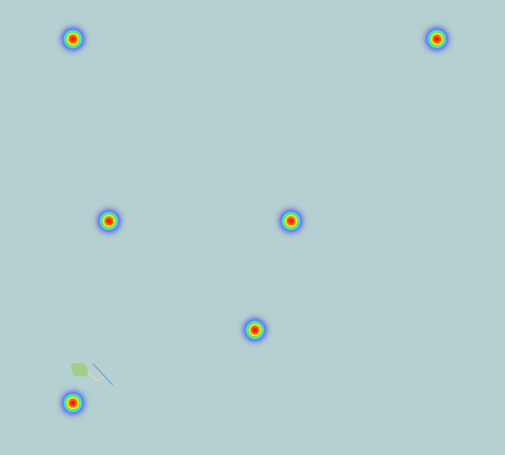
\includegraphics[width=\textwidth]{plots/synthetic_base.png}
    \caption{Original synthetic data.}
    \label{fig:synth_origin}
\end{figure}

\begin{figure}[H]
    \centering
    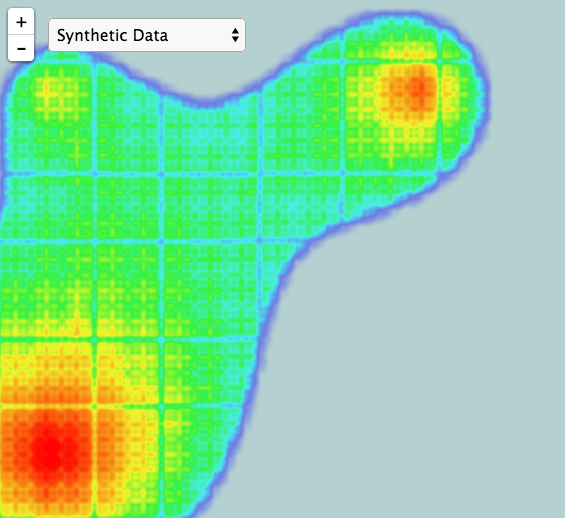
\includegraphics[width=\textwidth]{plots/synthetic_sample.png}
    \caption{Expected occupancy time using synthetic data.}
    \label{fig:synthetic}
\end{figure}

%%%%%%%%%%%%%%%%%%%%%%%%%%%%%%%
\subsection{Google Location API}
%%%%%%%%%%%%%%%%%%%%%%%%%%%%%%%

Many people use Android phones for navigation using the GPS, and Google Maps for finding out about places. What most of them are unaware of is that Google Inc. keeps a log of all places a person has visited while the GPS is active - what they call the Location History. Users can browse where they've been on a map. This used to be available through Google Latitude API, but it was closed down some time ago; it's still possible, though, to get the data through Google Takeout.

In this experiment, the author downloaded his own Location History in order to build a BBMM of himself. The data Google offers coms in the JSON format, with lots of additional information such as whether or not the person was actively moving during certain periods of time. The given Javascript code \texttt{parse\_location.js} can convert such JSON file into a TSV (tab-separated values) file, containing just a list of GPS coordinates in the E7 format together with absolute timestamps in milliseconds.

The results are again on the web visualizer, selecting the Google Latitude Data source. A snapshot is provided here for convenience.

\begin{figure}[H]
    \centering
    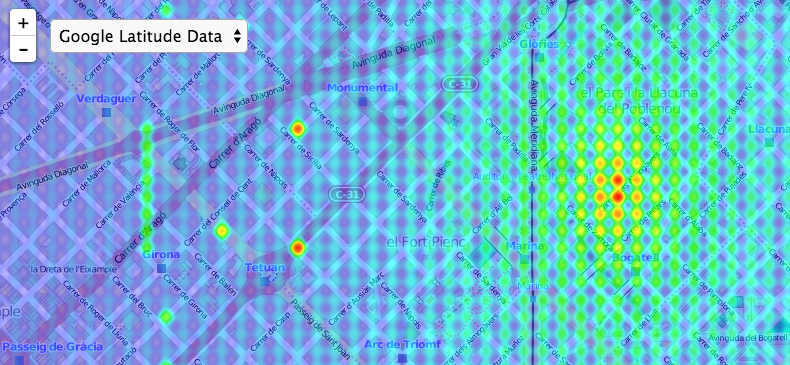
\includegraphics[width=\textwidth]{plots/google_sample.png}
    \caption{Expected occupancy time using data from Google Location History.}
    \label{fig:google_sample}
\end{figure}

% \begin{verbatim}
%     - google offers timestamped gps records for your user, internally used in google maps etc
%     - data avilable through Google Takeout
%     - data is formatted in JSON, with lots of metadata
%     - timestamps are in Unix epoch ms, gps in E7 format
%     - present results in the web visualizer
% \end{verbatim}

%%%%%%%%%%%%%%%%%%%%%%%%%%%%%%%
\subsection{Movebank Database}
%%%%%%%%%%%%%%%%%%%%%%%%%%%%%%%

Movebank is a website specialized in collecting GPS tracks from animals and making them available for research; these tracks usually come from scientific papers that present results on them. Since they have a common CSV format easily parsable, we made a script for importing it into the BBMM and estimating the expected occupation time for each space differential.

The data Movebank offers contains, among other fields, the latitude and longitude (in decimal degrees) of the animal plus a timestamp in a text format, like: \texttt{2008-12-01 06:00:00.000}. Fortunately, MATLAB parses them natively.

It should be easy to modify the given \texttt{bbmm\_movebank.m} script to read another track; the CSV file saved at the bottom of the script can be dragged onto the web-based visualizer for exploration.

\begin{figure}[H]
    \centering
    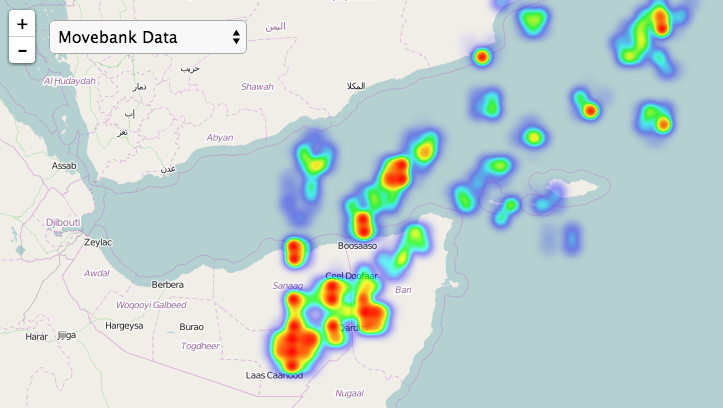
\includegraphics[width=\textwidth]{plots/movebank_sample.png}
    \caption{Expected occupancy time using data from Movebank.}
    \label{fig:movebank_sample}
\end{figure}

% \begin{verbatim}
%     - movebank offers timestapmed gps records for animals, normally released as part of scientific papers
%     - data is formated in CSV, from which we need to extract 3 relevant fields
%     - timestamps are in date format
%     - present results in the web visualizer
% \end{verbatim}

\clearpage
%%%%%%%%%%%%%%%%%%%%%%%%%%%%%%%
%%%%%%%%%%%%%%%%%%%%%%%%%%%%%%%
\section{Conclusion}
%%%%%%%%%%%%%%%%%%%%%%%%%%%%%%%
%%%%%%%%%%%%%%%%%%%%%%%%%%%%%%%

In this report, we described and presented an implementation of the Brownian Bridges Movement Model suitable for large datasets. All the code is available on GitHub \footnote{\url{https://github.com/lemonzi/brownian_bridges}}, including the MATLAB scripts, a pre-processing script in Javascript for the Google Latitude data, and the web-based visualization tool. The visualization tool is also live at \footnote{\url{https://lemonzi.github.io/brownian_bridges/web}}.

In general, BBMM is very useful when there are few known points; that is, it does a good job at interpolating. However, when there are lots of points close in time it does not really offer an edge compared to just assuming a normal distribution centered at the closest point.

The model has for sure room for improvement; a first thing one can think of is to stop assuming indenpendent brownian motion between pairs of points, and account for the fact that the animal has some momentum; for instance, by taking points in groups of 3 and performing a polynomial fitting of the mean instead of using a naïve linear interpolation.

% \begin{verbatim}
%     - remark the code is available on github, and it's possible to try it with different datasets
%     - brownian bridges are useful when there are few known points; they are good at interpolating, not at summarizing
%     - likewise, they perform poorly when extrapolating outside the defined time interval (they behave as regular brownian motion)
% \end{verbatim}

\end{document}